\documentclass[12pt]{article}

\usepackage[polish]{babel}
\usepackage{graphicx}
\usepackage{polski}
\usepackage[utf8]{inputenc}
\usepackage[section]{placeins}

\title{Raport z projektu SNR -- sieci głębokie w zastosowaniu do klasyfikacji obrazów zawierających numery budynków}
\author{
        Łukasz Neumann \\
            \and
        Witold Oleszkiewicz \\
}
\date{\today}

\begin{document}
\maketitle


\section{Wstęp}

Niniejszy raport przedstawia wyniki prac w ramach projektu z przedmiotu Sztuczne Sieci Neuronowe. Prezentujemy dane i oprogramowanie, które wykorzystaliśmy do zbudowania i przetrenowania głębokiej splotowej sieci neuronowej oraz wyniki walidacji tej sieci na zbiorze zdjęć cyfr oznaczających numery budynków. Dodatkowo zbadaliśmy wpływ użycia warstwy \textit{dropout} na jakość klasyfikacji.

\section{Dane}

Dane wykorzystane w danym projekcie są rzeczywistymi danymi, które pochodzą z obrazów Google Street View \cite{dane}. Na obrazach są widoczne tabliczki z numerami budynków. Wykorzystaliśmy zbiór po wstępnej obróbce, która polegała na znalezieniu na zdjęciach obszarów, na których widoczne są przede wszystkim cyfry składające się na numer budynku, których szerokość i wysokość są większe niż połowa szerokości i wysokości analizowanych zdjęć.

Każde ze zdjęć jest kolorowe oraz składa się z 32x32 pikseli. Do każdego ze zdjęć jest przyporządkowana etykieta, która oznacza cyfrę widoczną na zdjęciu (od 0 do 9). Wykorzystaliśmy dwa dostępne zbiory:

\begin{itemize}
\item zbiór trenujący, który składa się z 73257 zdjęć cyfr,
\item zbiór testujący, która składa się z 26032 zdjęć cyfr.
\end{itemize}

\section{Oprogramowanie}

Do budowania i trenowania głębokich sieci neuronowych zastosowaliśmy Keras \cite{keras} -- bibliotekę/API wysokiego poziomu w języku Python oraz bibliotekę Theano \cite{theano}, z której nie korzystaliśmy bezpośrednio, a posłużyła ona jako \textit{backend}. 

\section{Przygotowanie danych}

Zdjęcia skonwertowano z kolorowych na czarno-białe, gdyż kolor nie wpływa na klasyfikację cyfry.

Zamiast etykiet (od 0 do 9) dla każdego ze zdjęć, zastosowaliśmy wektor składający się z dziewięciu zera i jednej jedynki, która znajduje się na $i$-tej pozycji dla cyfry $i$.

\section{Architektura sieci głębokich i dodatkowy problem badawczy}

Zdefiniowaliśmy sieć neuronową składającą się z 12 warstw ukrytych (w tym 4 warstw splotowych):

\begin{tabular}{|r|c|c|c|}
  \hline 
  Warstwa & Wymiary wyjścia & Liczba parametrów & Opis\\
  \hline
  conv 2D & 30x30x32 & 320 & 32 maski 3x3\\
  \hline
  dropout & 30x30x32 &  & usunięcie 20\% neuronów \\
  \hline
  conv 2D & 28x28x32 & 9248 & 32 maski 3x3\\
  \hline
  max pool 2D & 14x14x32 &  & okno 2x2\\
  \hline
  conv 2D & 12x12x32 & 9248 & 32 maski 3x3\\
  \hline
  dropout & 12x12x32 &  & usunięcie 20\% neuronów \\
  \hline
  conv 2D & 10x10x32 & 9248 & 32 maski 3x3\\
  \hline
  max pool 2D & 5x5x32 &  & okno 2x2\\
  \hline
  flatten & 800 &  & \\
  \hline
  dense & 512 & 410112 & \\
  \hline
  dropout & 512 &  & usunięcie 50\% neuronów \\
  \hline
  dense & 10 & 5130 & \\
  \hline

\end{tabular} 

Jako funkcję aktywacji neuronów użyto funkcję ReLU: $a(x) = \max(0, x)$. Wartość normy wag została ograniczona do $3$. W warstwie wyjściowej zastosowano funkcję \textit{softmax}: $\sigma(z)_j=\frac{\exp{z_j}}{\sum_k \exp(z_k)}$.

Do optymalizacji sieci neuronowej wybrano algorytm stochastycznego spadku gradientu z parametrami momentum:$0.9$, decay:$0.0004$, learning rate:$0.04$. Optymalizację przeprowadzano przez 100 epok, gradient obliczano na podstawie 128 zdjęć ze zbioru trenującego. Zastosowano funkcję celu, entropia krzyżowa: $y\log a + (1-y)\log(1-a)$, gdzie $a$ to wartość wyjścia a $y$ to oczekiwana wartość wyjścia.

Dodatkowym problemem badawczym było przeanalizowanie wyników walidacji powyższej sieci neuronowej w zależności od warstwy \textit{dropout}. Warstwa \textit{dropout}, to warstwa, która nie bierze pod uwagę niektóre (losowe) wyjścia neuronów warstwy poprzedzającej. Analizowaliśmy jakość klasyfikacji bez warstwy \textit{dropout}, z warstwą \textit{dropout} tak jak w powyższej sieci (ten przypadek będzie nazywany dużym \textit{dropout'em}) oraz z warstwą \textit{dropout} o współczynnikach mniejszych o połowę, czyli usnięcie $10\%$ neuronów po warstwach konwolucyjnych oraz $25\%$ neuronów po warstwie dense (ten przypadek będzie nazywany małym \textit{dropout'em}).

\section{Wyniki}

Na wykresach \ref{acc_no_dropout}, \ref{acc_half_dropout} i \ref{acc_dropout} przedstawiono dokładność klasyfikacji cyfr ze zdjęć Google Street View w czasie uczenia się sieci neuronowej (bez \textit{dropout'em}, z małym \textit{dropout'em} i z dużym \textit{dropout'em}) przez 100 epok. Dokładność klasyfikacji była liczona na dwóch zbiorach: na zbiorze trenującym oraz na zbiorze testowym, który nie był używany w procesie uczenia się sieci.

Na wykresie \ref{acc_no_dropout} widzimy, że dokładność na zbiorze trenującym już po 20 epokach wynosi około $99.9\%$, natomiast na zbiorze testującym dokładność po około 6 epokach stabilizuje się na poziomie około $89.8\%$.

Na wykresie \ref{acc_dropout} można zaobserwować, jak dodanie do sieci warstw typu \textit{dropout} wpływa na jakość klasyfikacji. Osiągnięta po 100 epokach dokładność klasyfikacji cyfr mierzona na zbiorze trenującym jest mniejsza niż w poprzednim przypadku ($99.9\%$) i wynosi około $97.5\%$ (przy czym po 100 epokach wciąż wykazuje mały wzrost, więc być może po większej liczbie epok ta dokładność byłaby większa). Jednakże dla sieci z \textit{dropout'em} dokładność na zbiorze testującym jest wyższa niż dla poprzedniego przypadku ($89.8\%$) i wynosi około $92.8\%$ po 100 epokach. Jest to wynik podobny do wyniku opisanego w pracy referencyjnej \cite{reference-paper} (lepsze wyniki -- około $96\%$ dokładności --uzyskano dla sieci jedenastowarstwowej).

Dla mniejszego \textit{droput'u} (wykres \ref{acc_half_dropout}) osiągnięto lepszą dokładność ($91.3\%$) niż bez warstwy \textit{dropout}, ale mniej niż dla sieci z większym \textit{dropout'em.} 

Dodanie warstw \textit{dropout} do naszej sieci neuronowej dało lepszą dokładność klasyfikacji na zbiorze testowym i gorszą dokładność na zbiorze trenującym, co oznacza, że warstwa \textit{dropout} skutecznie walczy z nadmiernym dopasowaniem się do zbioru trenującego i pozwala uzyskać lepszą generalizacje.

Na wykresach \ref{loss_no_dropout}, \ref{loss_half_dropout} i \ref{loss_dropout} przedstawiono wartość funkcji celu w czasie uczenia się sieci neuronowej. Dla sieci bez warstwy \textit{dropout} funckja celu na zbiorze trenującym osiąga minimum (zero) już po około 20 epokach, lecz niestety na zbiorze testującym wartość funkcji celu odbija się od wartości $0.4$ po około 5 epokach i następnie rośnie, by ustabilizować się na poziomie około $0.9$ po 30 epokach. W przeciwieństwie do tej sieci, sieci z warstwami \textit{dropout} lepiej minimalizują funkcję celu, nie obserwujemy też odbicia dużego odbicia się wartości funkcji celu (trochę większe odbicie jest dla sieci z mniejszym \textit{dropout'em}). Po 100 epokach wartość funkcji celu mierzona na zbiorze testującym wynosi około $0.55$ dla sieci z małym \textit{dropout'em} i około $0.35$ dla sieci z dużym \textit{dropout'em}.

Porównując wykresy \ref{loss_no_dropout}, \ref{loss_half_dropout} i \ref{loss_dropout} wnioskujemy, że zastosowanie warstwy \textit{dropout} pozwoliło uniknąć nadmiernego dopasowania do zbioru trenującego i dzięki temu udało się osiągnąć lepsze minimum na zbiorze testującym.


\begin{figure}[!ht]
\centering
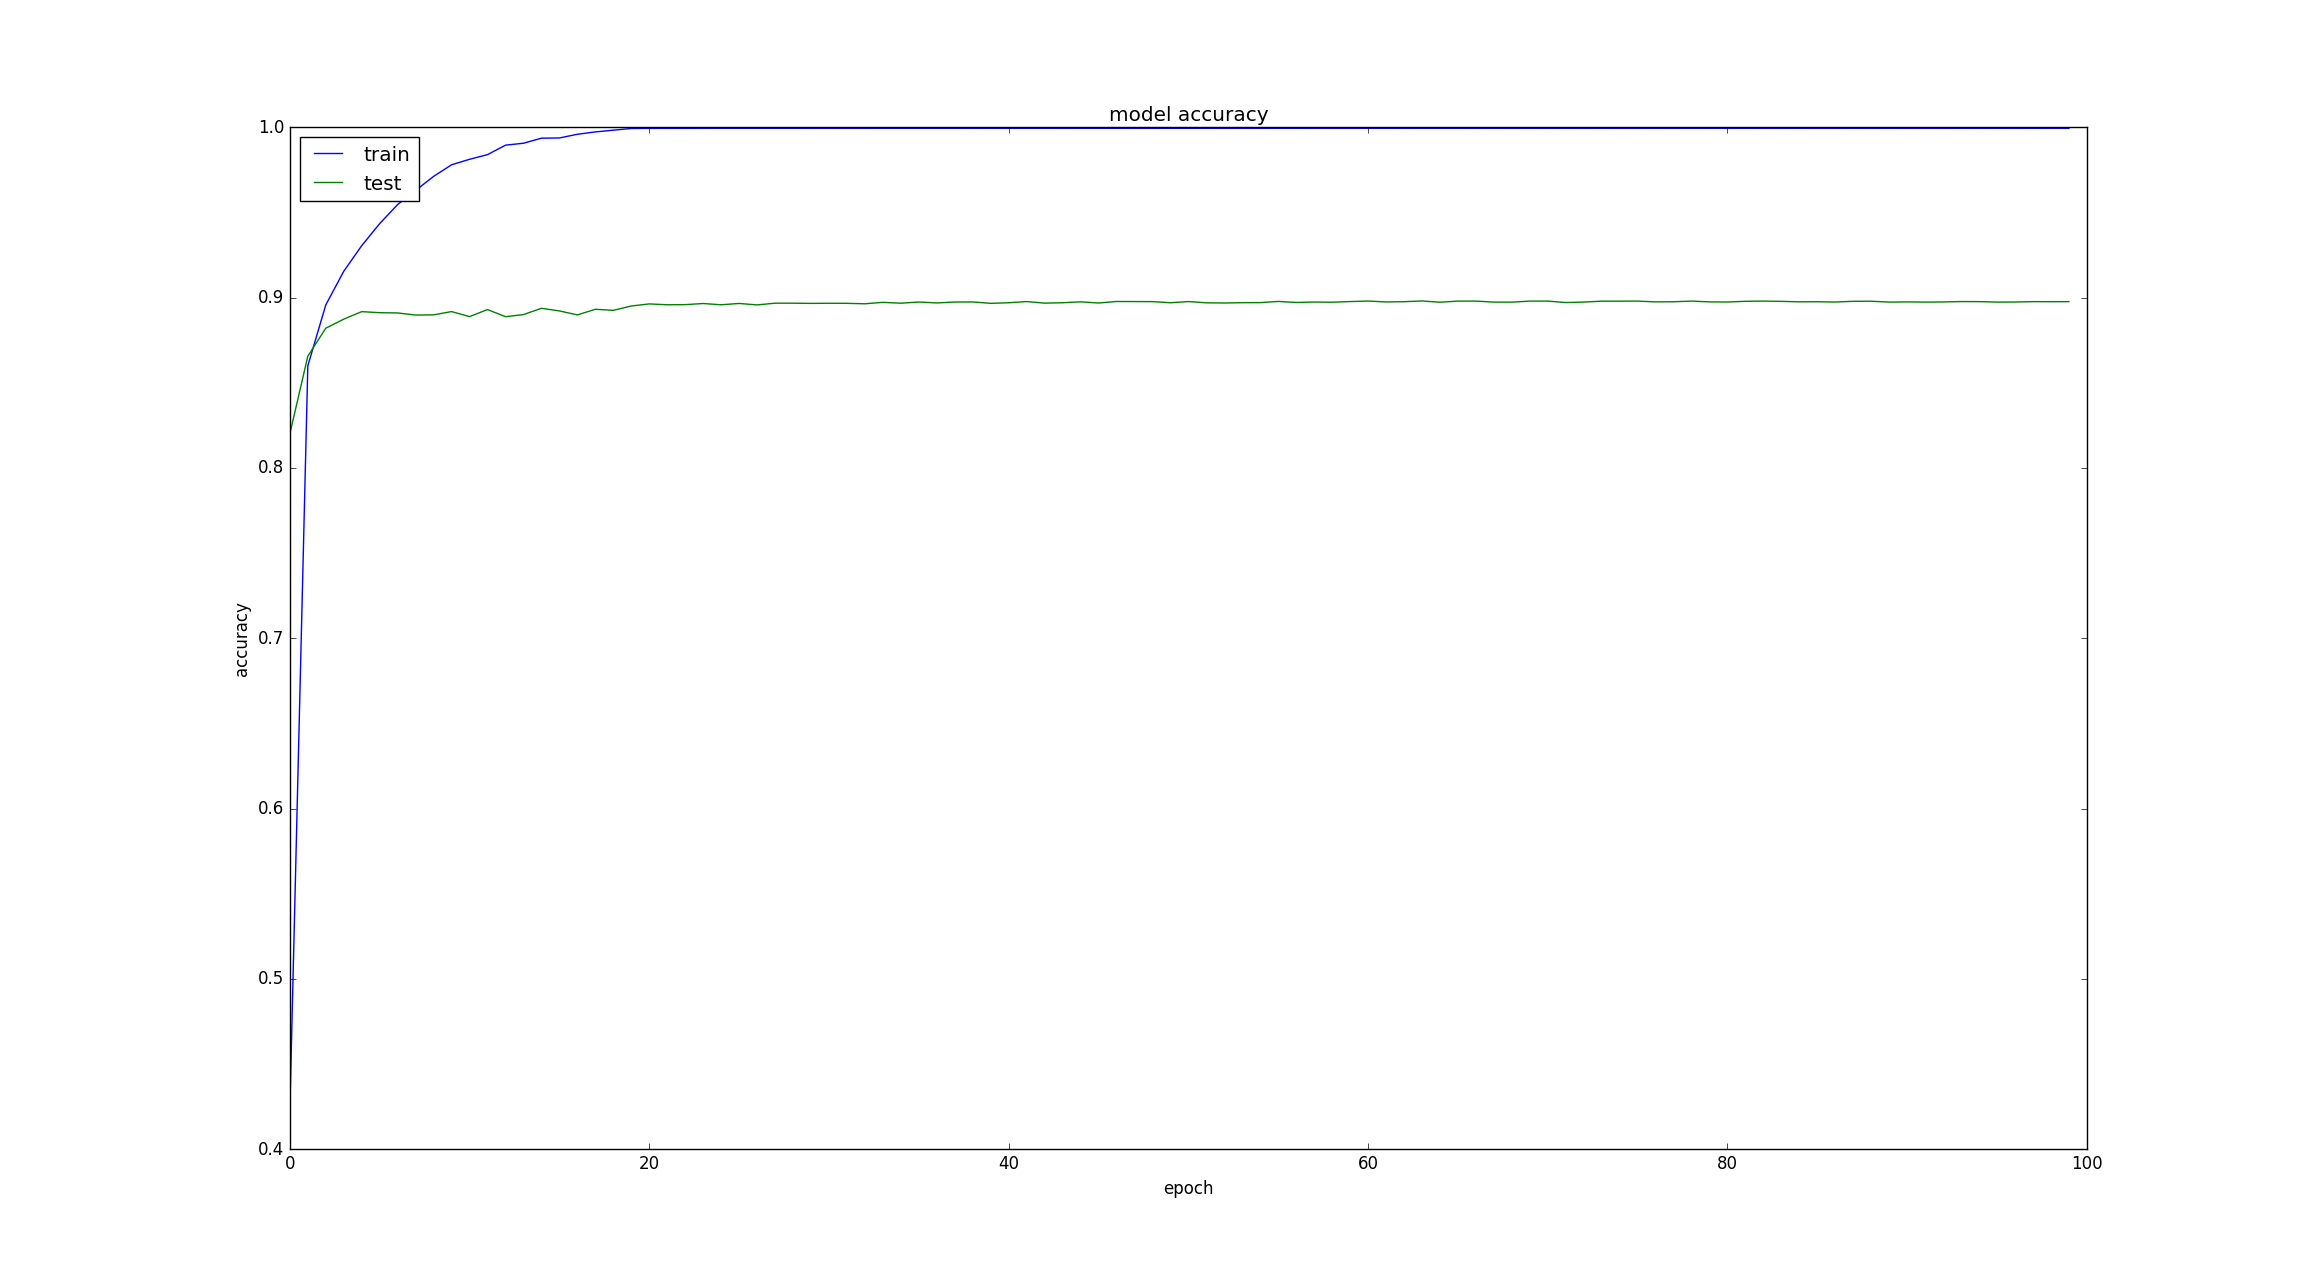
\includegraphics[scale=0.25]{acc_no_dropout}
\caption{Dokładność klasyfikacji dla sieci neuronowej bez \textit{dropout'u}.}
\label{acc_no_dropout}
\end{figure}


\begin{figure}[!ht]
\centering
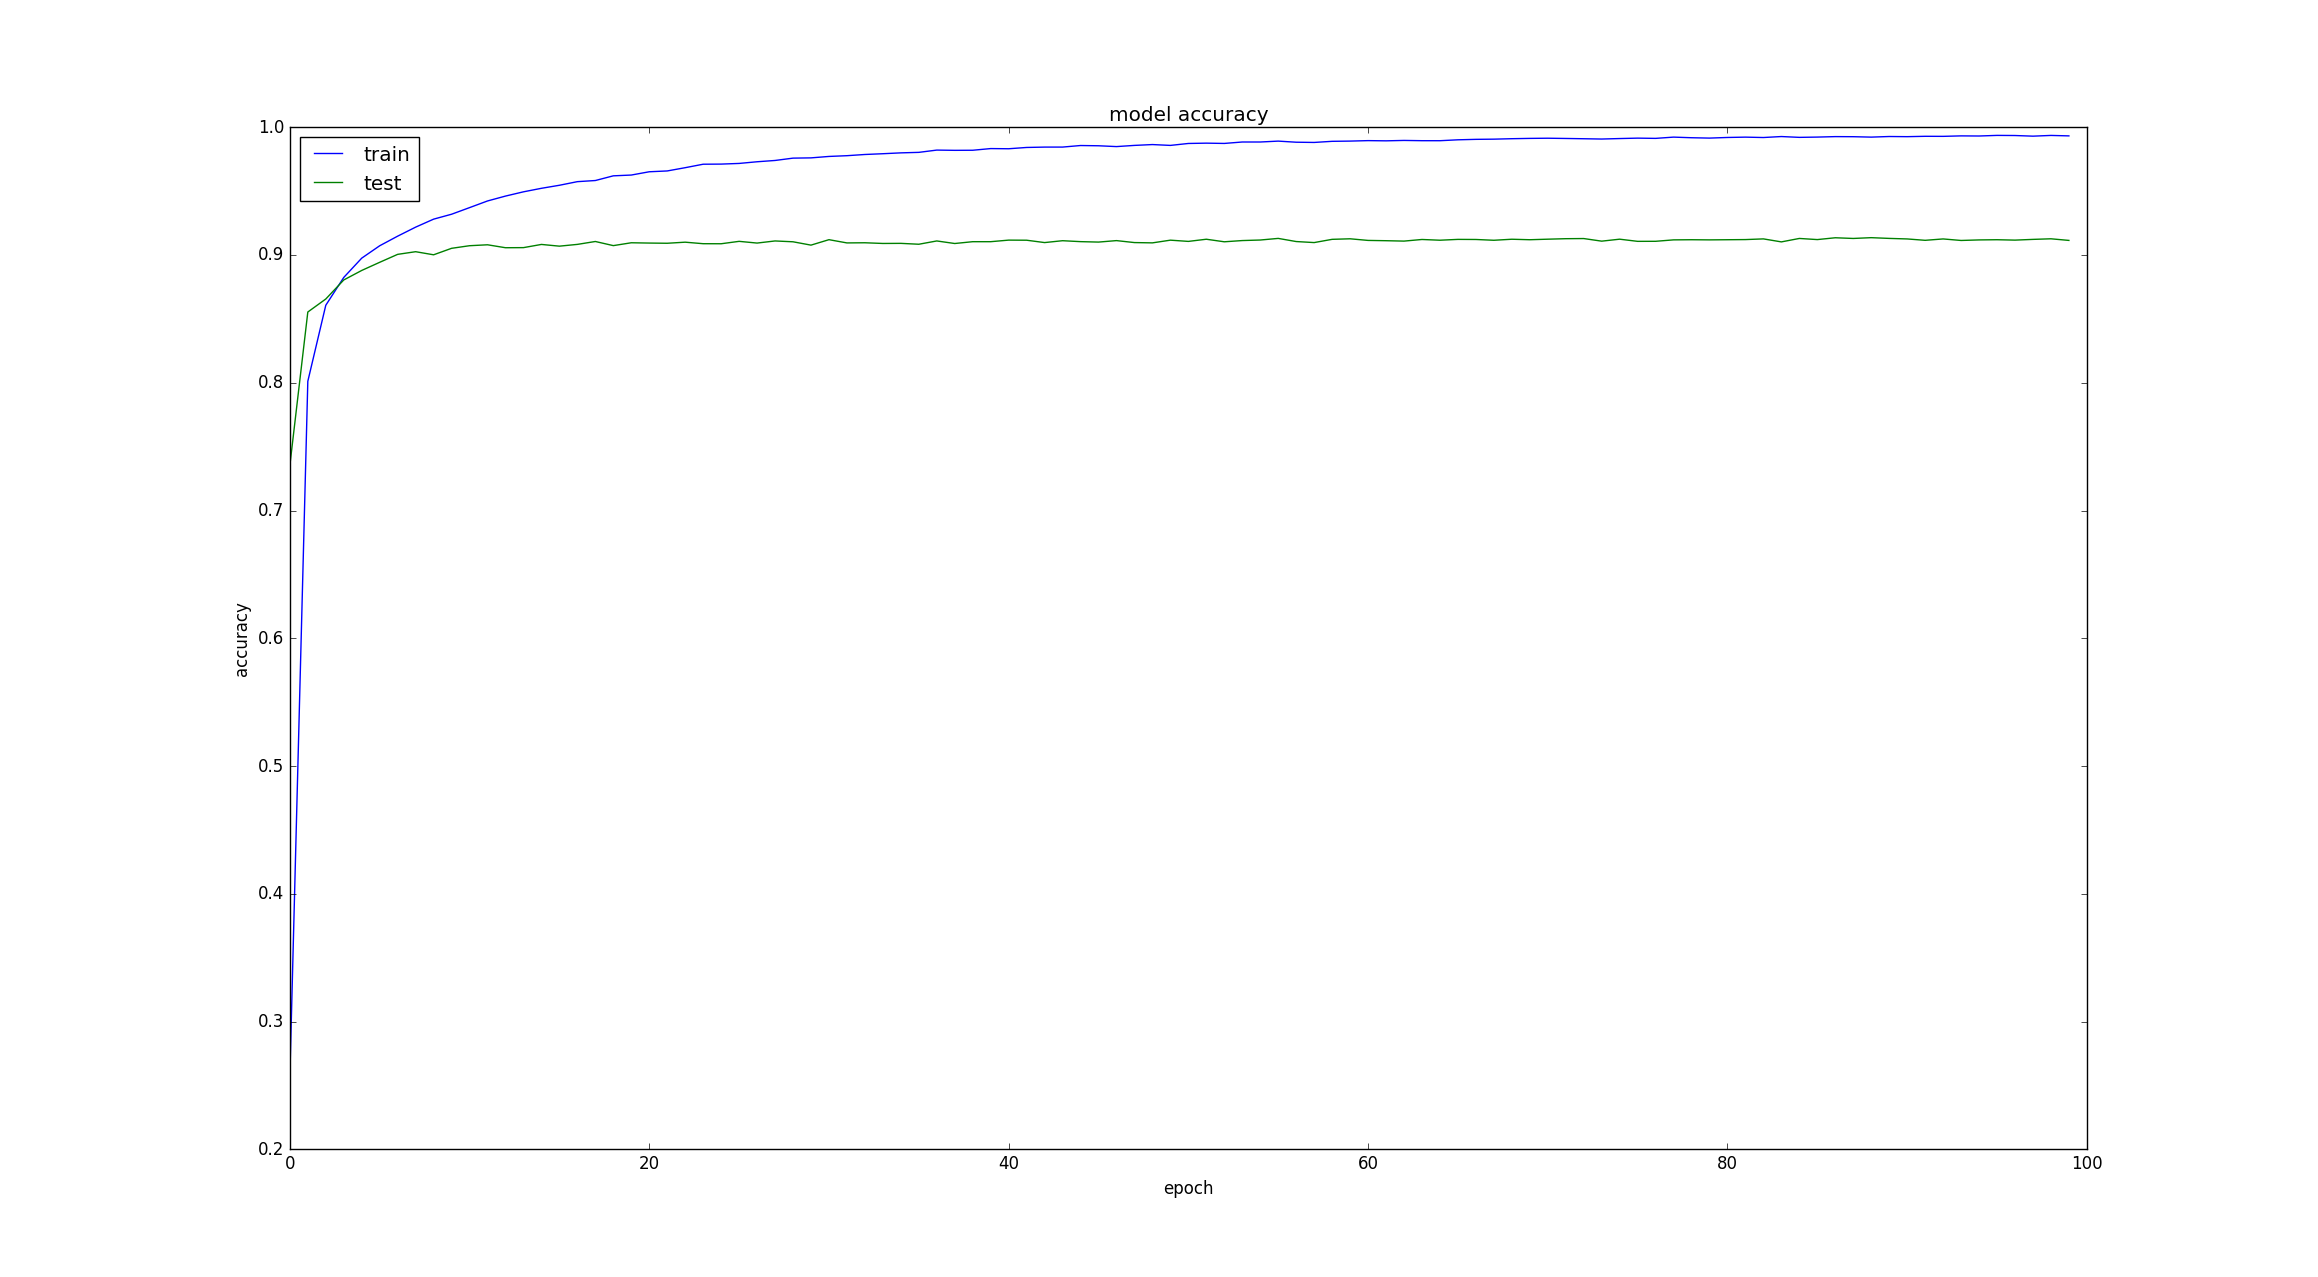
\includegraphics[scale=0.25]{acc_half_dropout}
\caption{Dokładność klasyfikacji dla sieci neuronowej z małym \textit{dropout'em}.}
\label{acc_half_dropout}
\end{figure}

\begin{figure}[!ht]
\centering
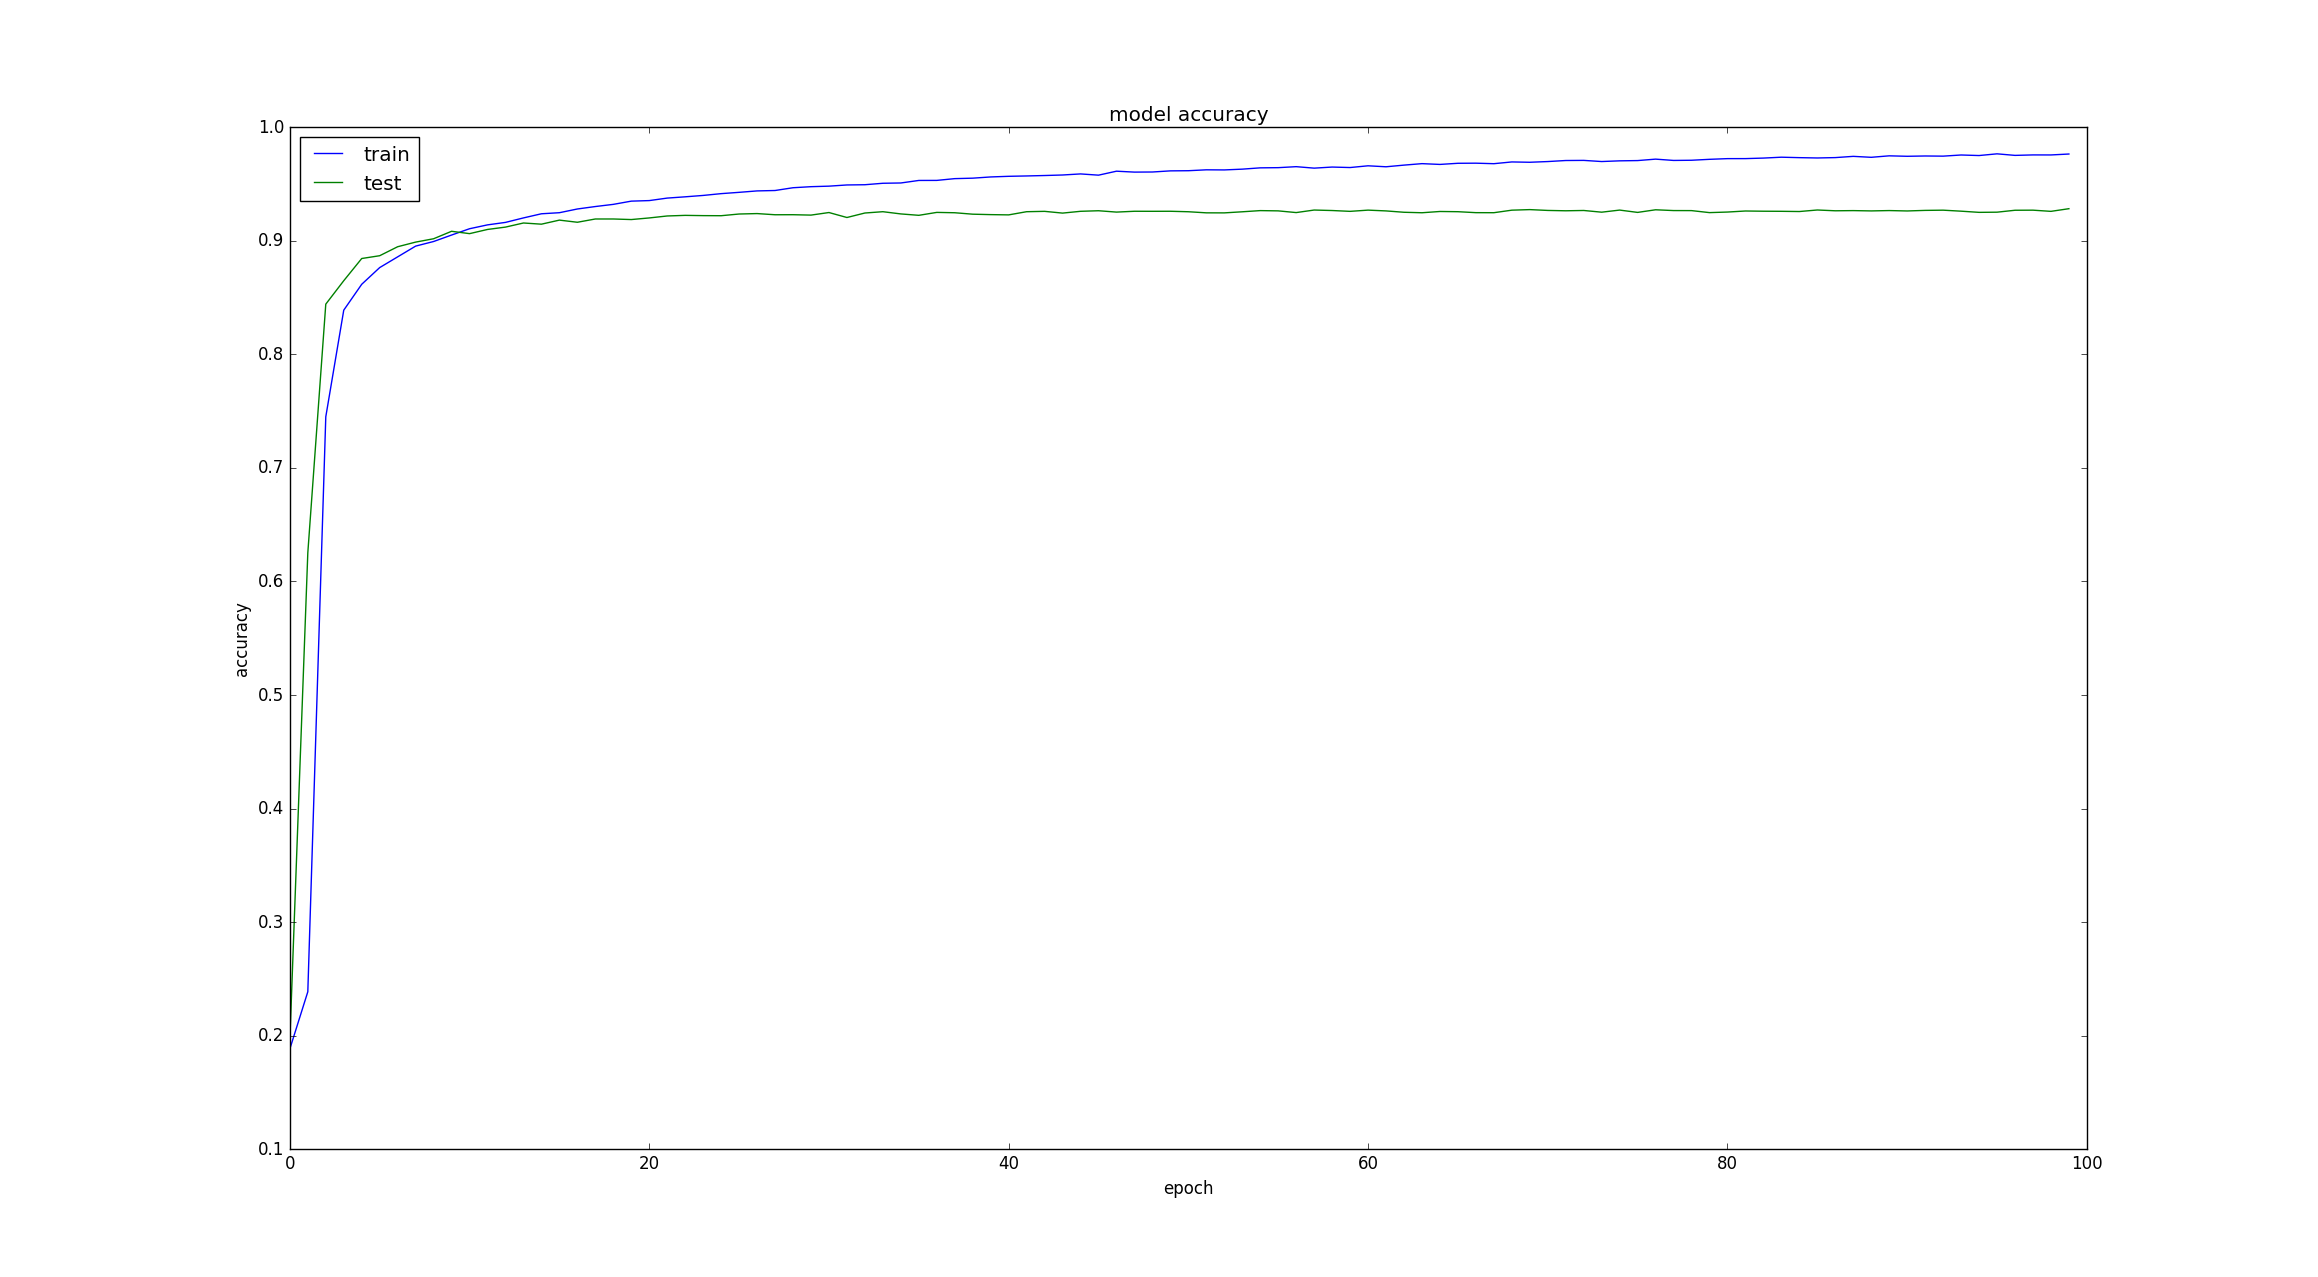
\includegraphics[scale=0.25]{acc_dropout}
\caption{Dokładność klasyfikacji dla sieci neuronowej z dużym \textit{dropout'em}.}
\label{acc_dropout}
\end{figure}

\begin{figure}[!ht]
\centering
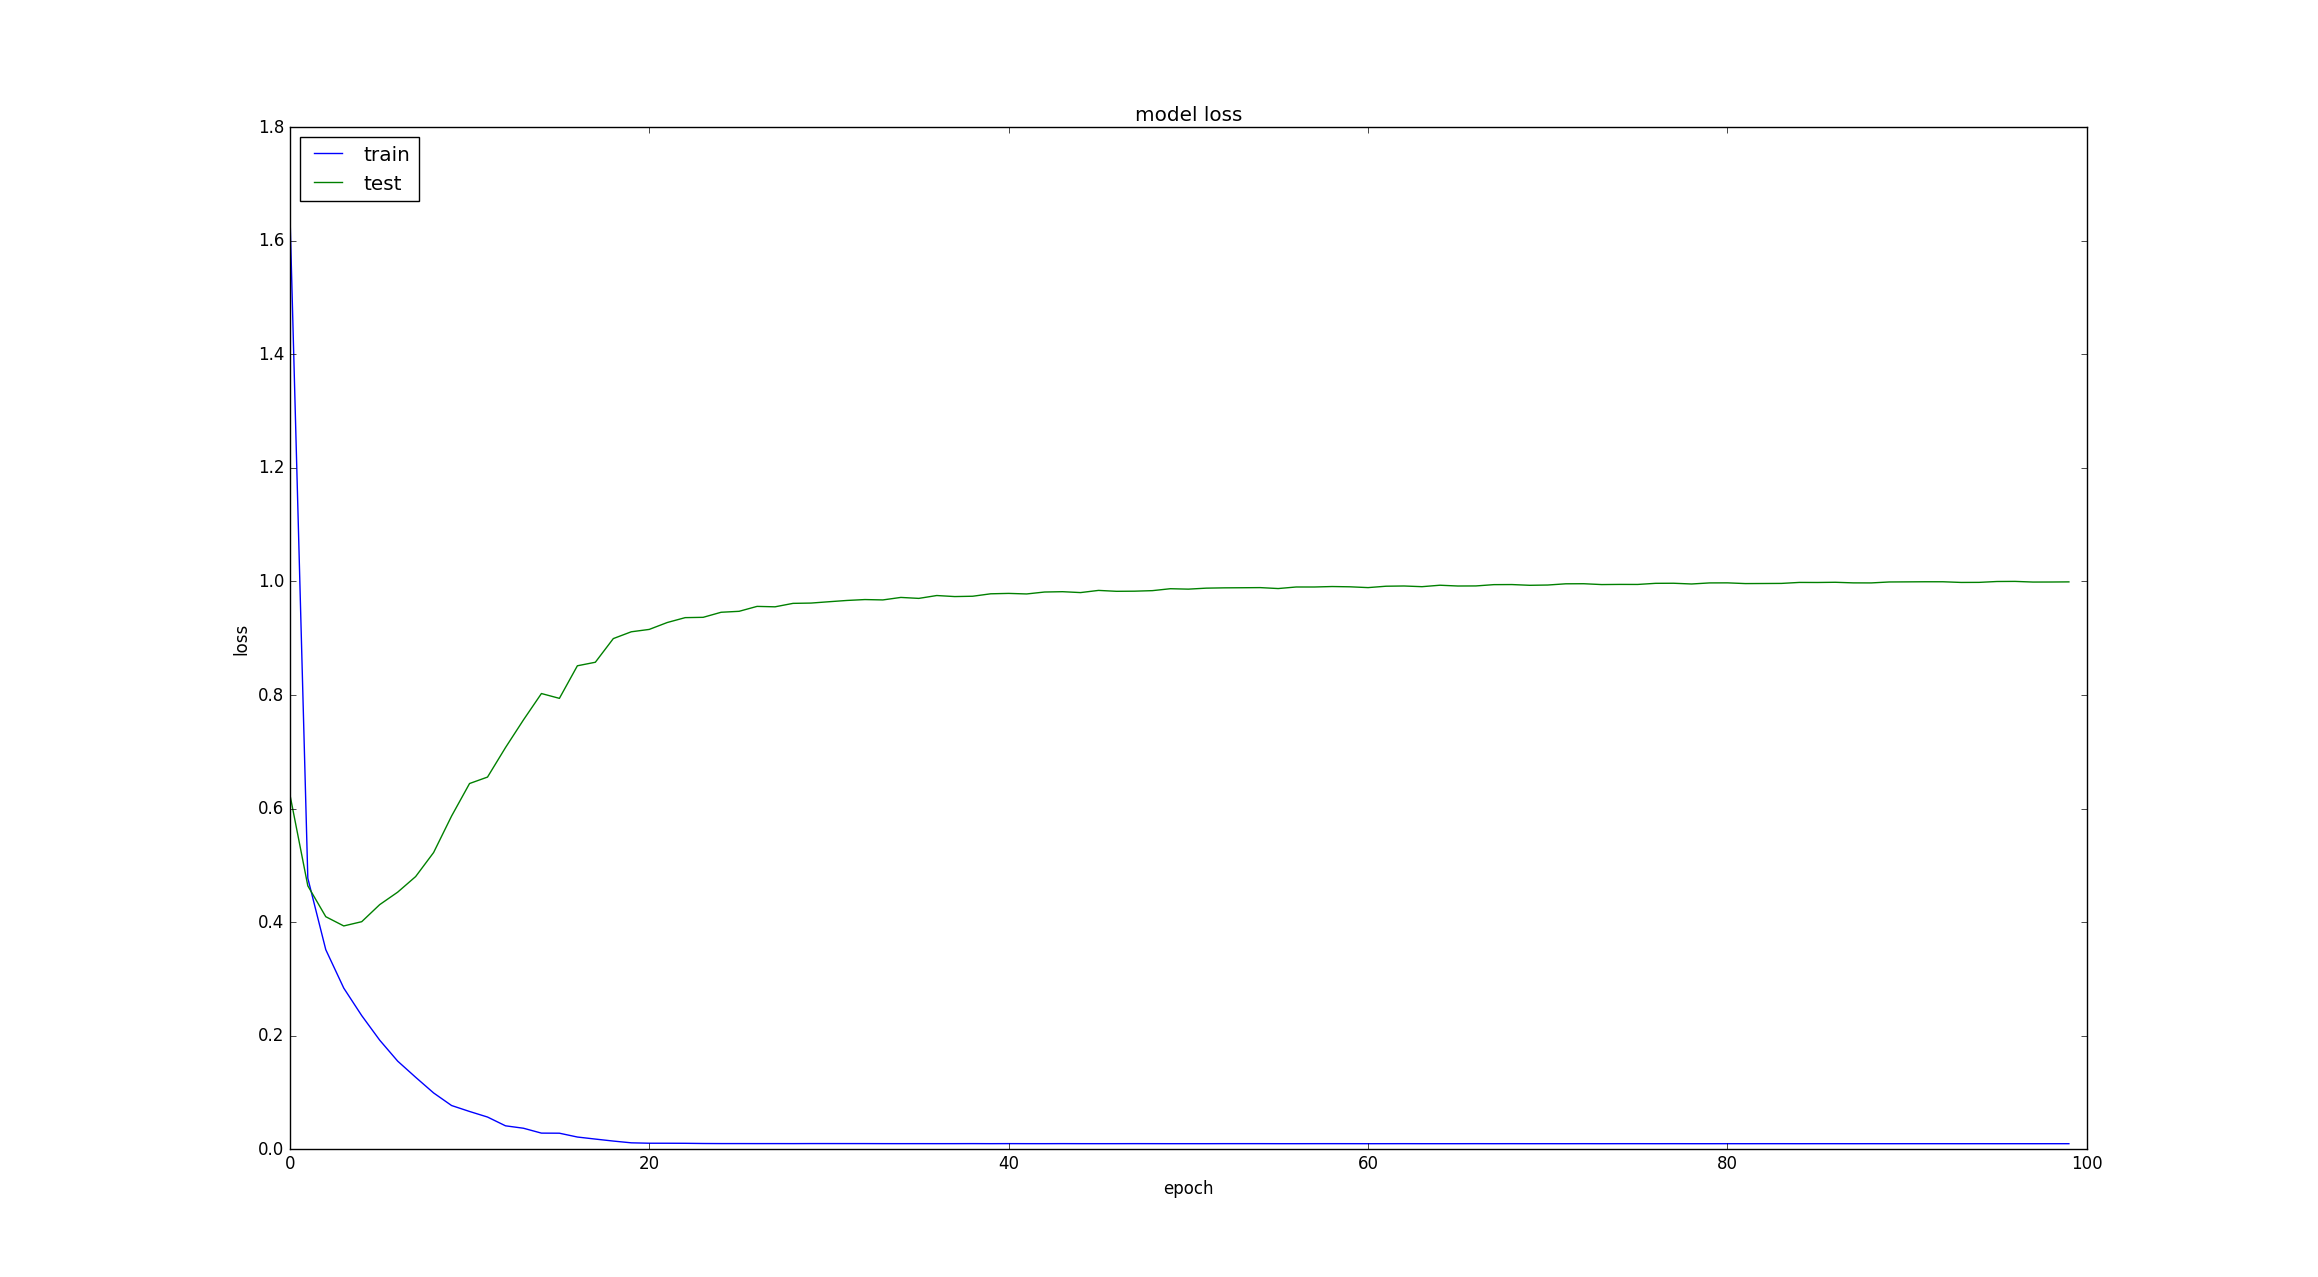
\includegraphics[scale=0.25]{loss_no_dropout}
\caption{Funkcja celu dla głębokiej sieci neuronowej bez \textit{dropout'u}.}
\label{loss_no_dropout}
\end{figure}

\begin{figure}[!ht]
\centering
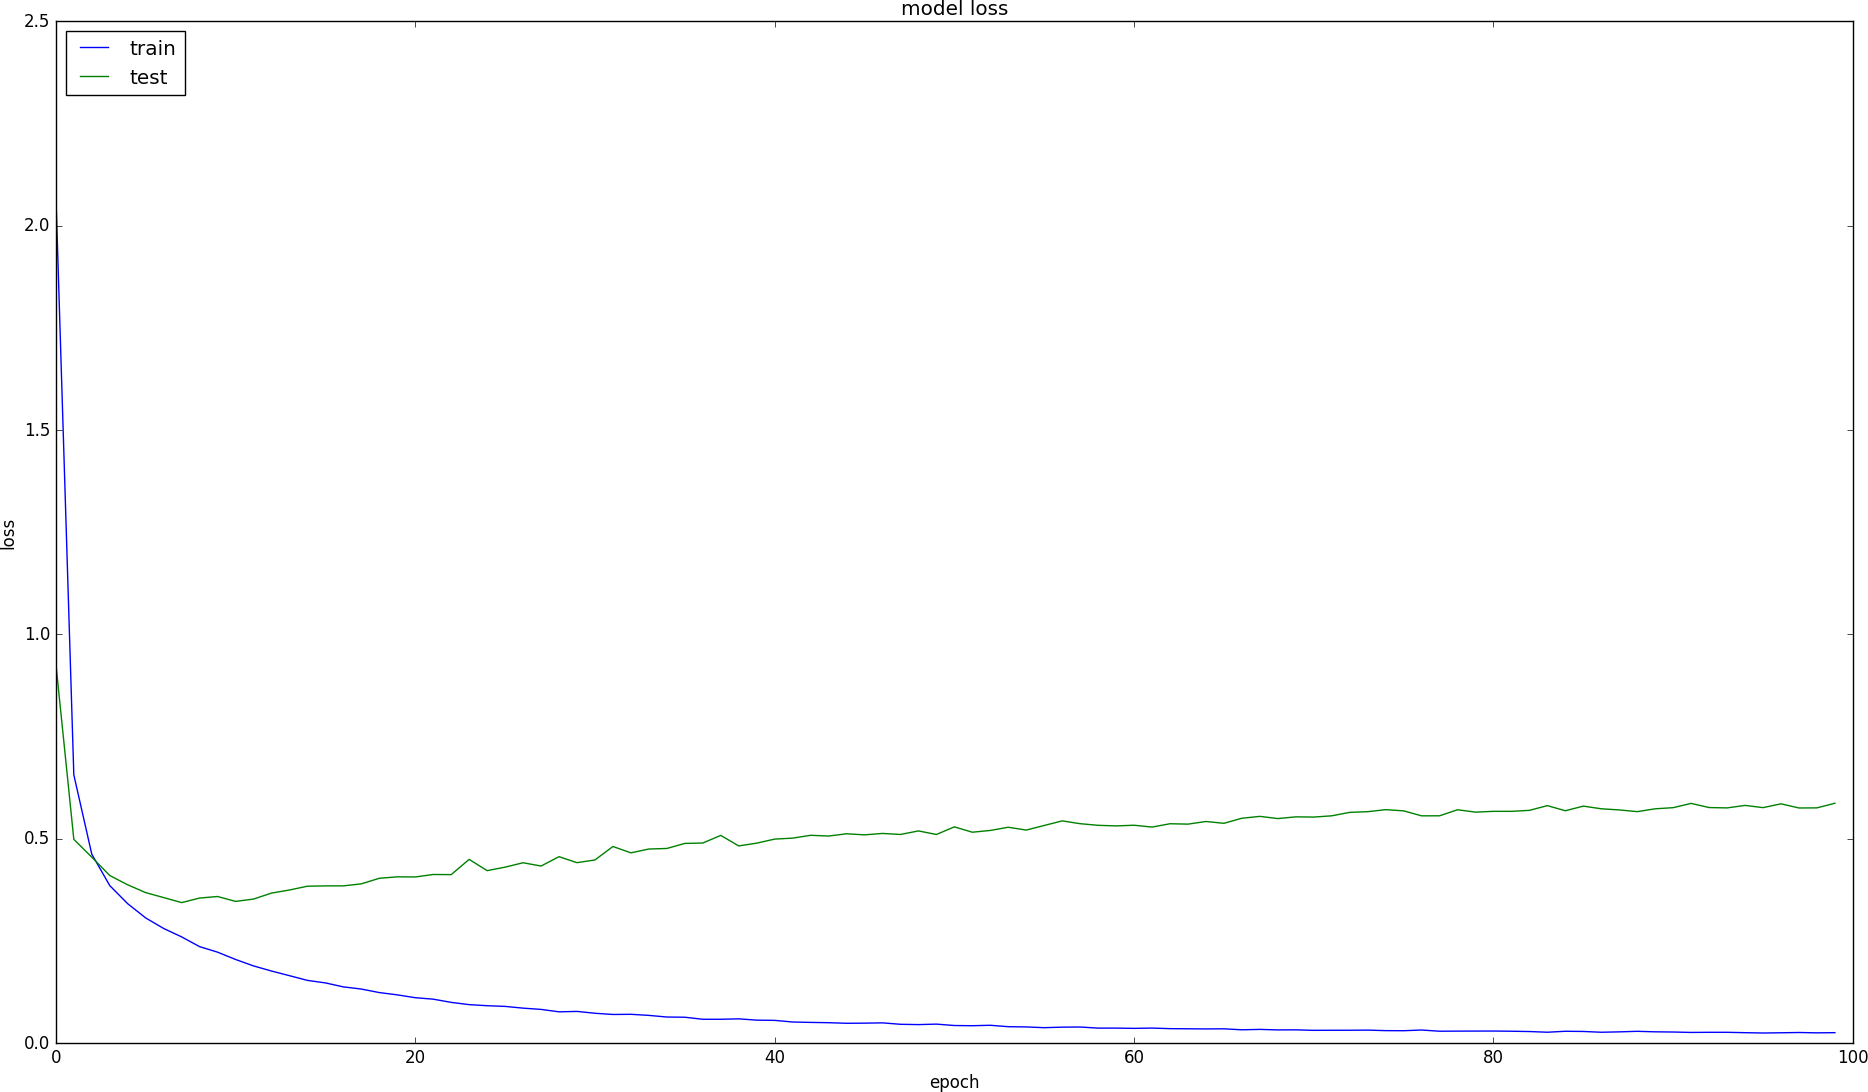
\includegraphics[scale=0.25]{loss_half_dropout}
\caption{Funkcja celu dla głębokiej sieci neuronowej z małym \textit{dropout'em}.}
\label{loss_dropout}
\end{figure}


\begin{figure}[!ht]
\centering
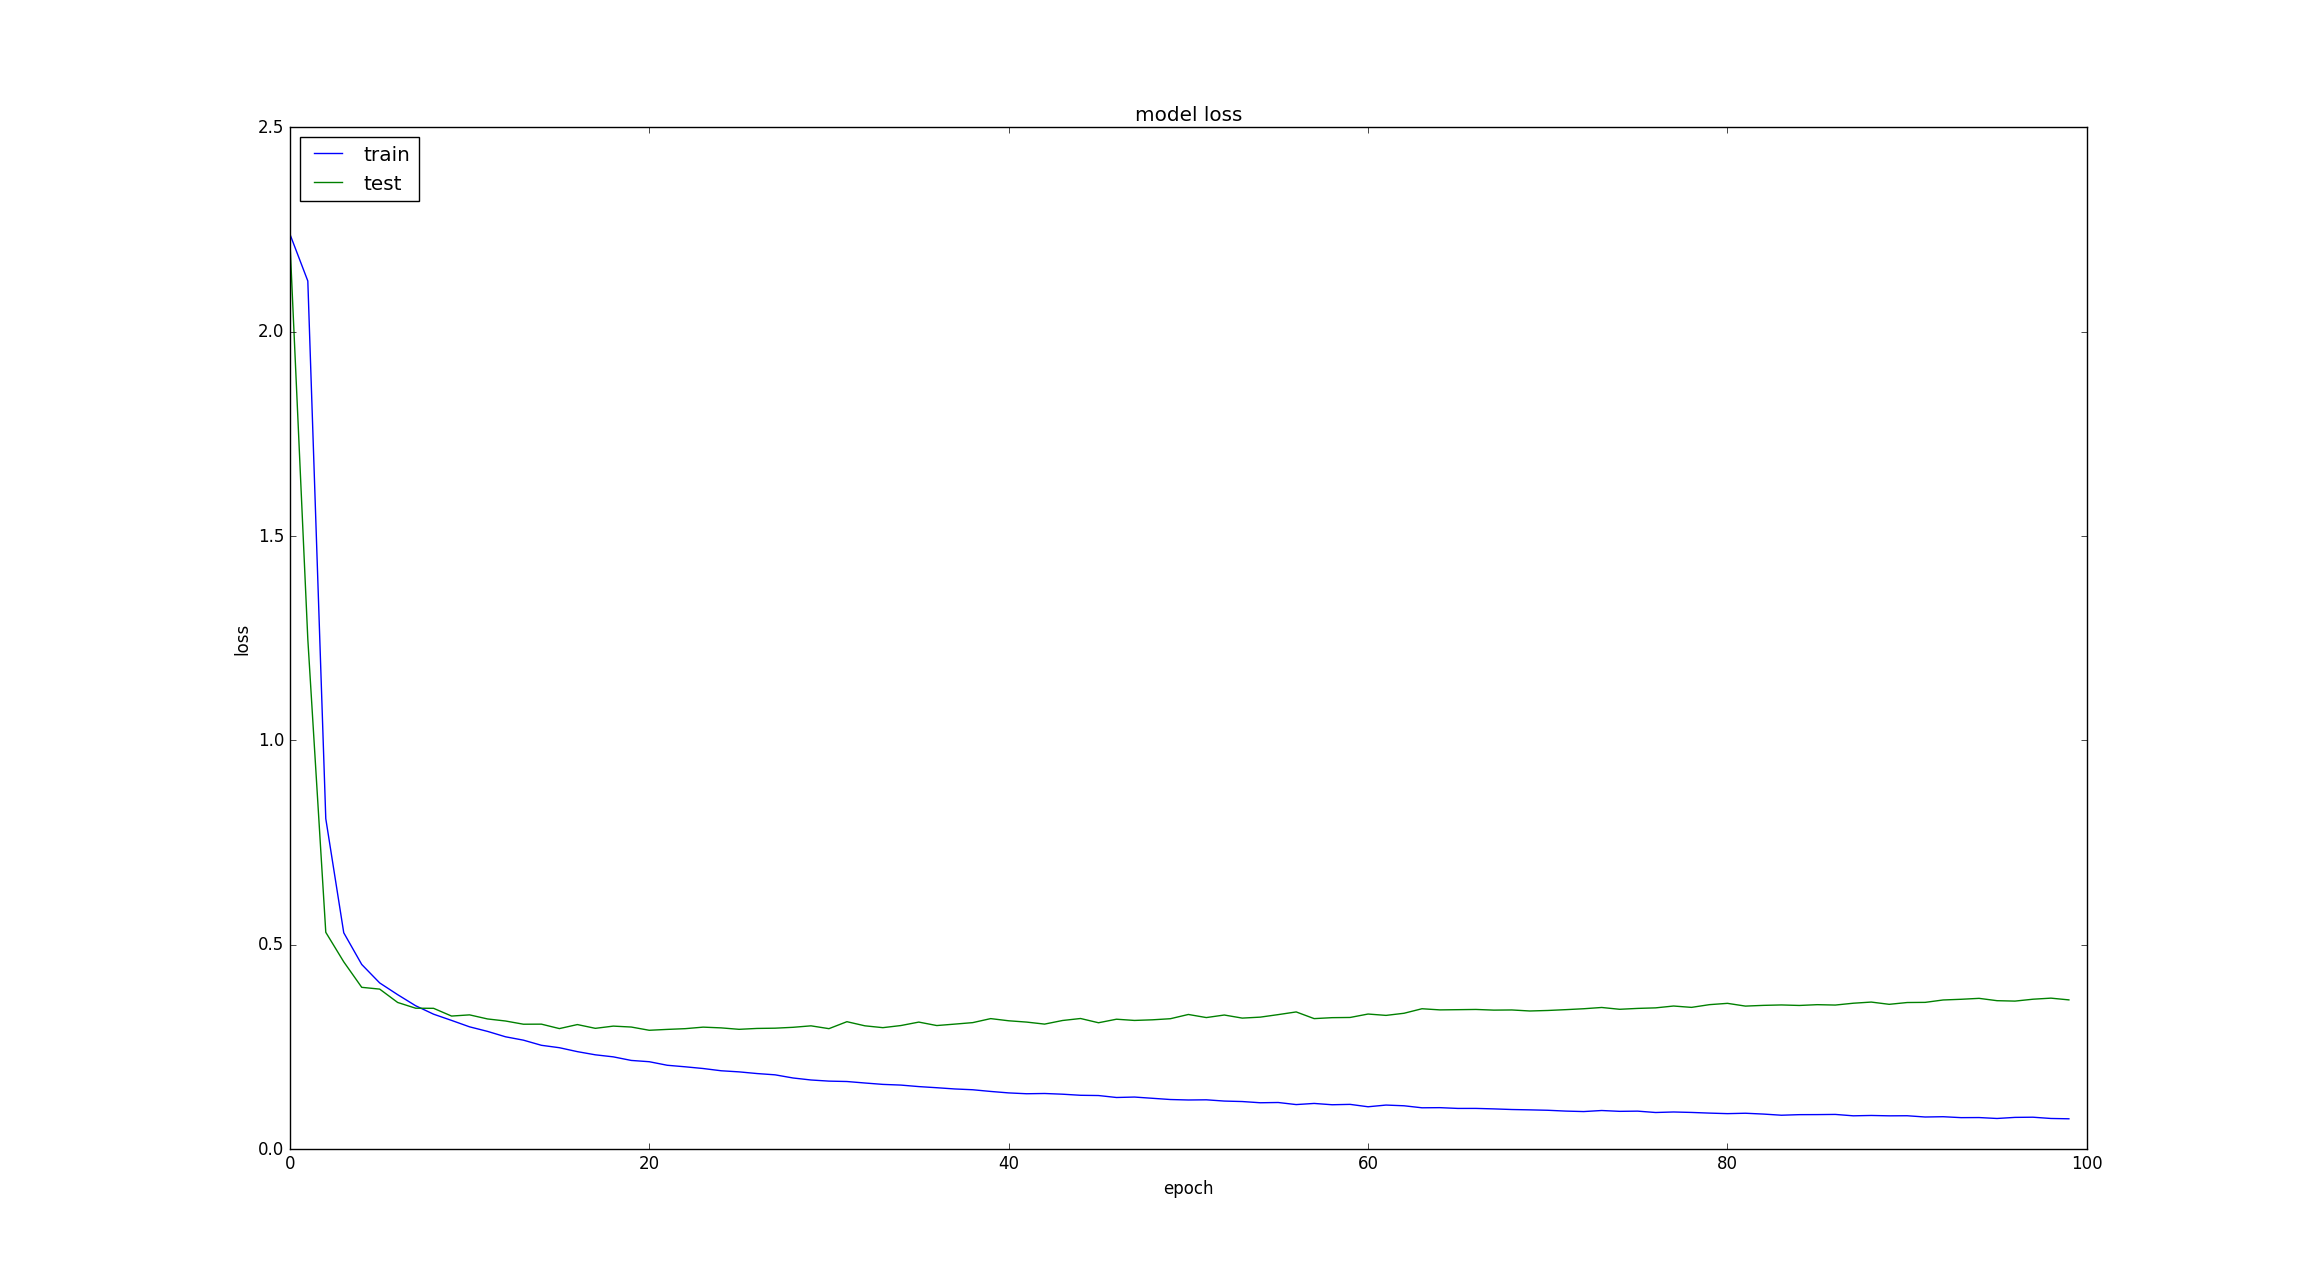
\includegraphics[scale=0.25]{loss_dropout}
\caption{Funkcja celu dla głębokiej sieci neuronowej z dużym \textit{dropout'em}.}
\label{loss_dropout}
\end{figure}

\begin{thebibliography}{9}

\bibitem{dane}
The Street View House Numbers (SVHN) Dataset,
Yuval Netzer, Tao Wang, Adam Coates, Alessandro Bissacco, Bo Wu, Andrew Y. Ng
Reading Digits in Natural Images with Unsupervised Feature Learning NIPS Workshop on Deep Learning and Unsupervised Feature Learning
2011
http://ufldl.stanford.edu/housenumbers/

\bibitem{keras}
https://keras.io

\bibitem{theano}
http://deeplearning.net/software/theano/

\bibitem{reference-paper}
Ian J. Goodfellow, Yaroslav Bulatov, Julian Ibarz, Sacha Arnoud, Vinay D. Shet
"Multi-digit Number Recognition from Street View Imagery using Deep Convolutional Neural Networks",
CoRR (2013)


\end{thebibliography}

\end{document}
